\documentclass[10pt, a4paper]{article}

%Preambuła dokumentu
\usepackage{graphicx}
\usepackage{here}
\usepackage{rotating}
\usepackage{subfigure}
\usepackage{epic}
\usepackage{listings}
\usepackage{verbatim}
\usepackage{amssymb}
\usepackage{amsmath}
\usepackage[polish]{babel}
\usepackage[OT4]{fontenc}
\usepackage[utf8]{inputenc}

%\usepackage{here}

\textwidth      16cm
\textheight     25.5cm
\evensidemargin -3mm
\oddsidemargin  -3mm
\topmargin      -20mm



\author{Marcin Ciopcia \and Daniel Gut \and Piotr Semberecki \and Hanna Sienkiewicz \and Mateusz Stachowski
}
 
\title{Raport z projektu Systemy Zdarzeniowe} 

\date{\today}

\begin{document}
\maketitle



\section{Problem Projektu}
\label{sec:wstep}
%
\subsection{Opis ogólny}
Pierwszym celem projektu jest symulacja zautomatyzowanej linii produkcyjnej z wieloma gniazdami wytwórczymi, obsługiwanej przez wózki AGV. Linia produkcyjna ma kształt pierścienia, z ustalonym dozwolonym kierunkiem ruchu wózków AGV, poruszających się jak na rysunku~\ref{fig:sch}.
 \begin{figure}[H]
  \begin{center}
    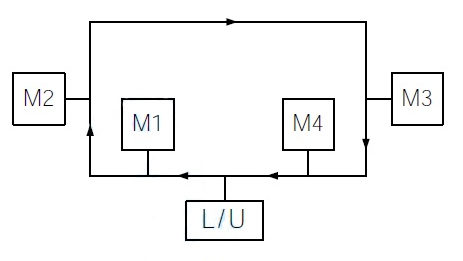
\includegraphics[width=0.3\textwidth]{./obrazki/Schemat.png}
    \caption{Struktura ścieżek}
    \label{fig:sch}
  \end{center}
 \end{figure}
Modelowany system posiada stacje załadowczo-rozładowczą (L/U), cztery stacje  maszynowe $(M_1,M_2,M_3,M_4)$, z których każda posiada bufor wejściowy i wyjściowy oraz robota wykonującego operację przeniesienia detalu z bufora wejściowego na stanowisko robocze maszyny oraz ze stanowiska roboczego do bufora wyjściowego. Opisywany system produkcyjny realizuje współbieżnie do sześciu typów produktów w podanej ilości. Operacje na danym produkcie zostają wykonane na rożnych maszynach w zadanej kolejności.
 
 
Następnie zostanie opracowany sterownik zdarzeniowy zarządzający logiką przepływu zadań w systemie składającą się z
\begin{itemize}
\item klasyfikatora zadań możliwych do realizacji,
\item systemu agentowego zarządzającego kolejnością wykonywania działań,
\item systemu przeciwdziałania zakleszczeniom zdarzeń w systemie.
\end{itemize}
Sterownik nadrzędny opisany zostanie za pomocą sieci Petriego, następnie zostanie oprogramowany w środowisku \textit{Matlab}.

\subsection{Zastosowanie systemów zdarzeniowych}
Podjęcie tego zagadnienie jest ważne ze względu na poszerzające się zastosowanie robotyzacji w wielu dziedzinach gospodarki. Za pomocą elastycznych komórek produkcyjnych (ESP) można modelować procesy produkcyjne, przepustowość sieci infrastruktury technicznej, systemy czasu rzeczywistego  \cite{scr} , sterowniki logiczne \cite{sl} czy sieć komunikacji miejskiej. Modele różnorodnych systemów pozwalają ocenić ich efektywność funkcjonowania \cite{mucha}, co może wpłynąć na zmniejszenie kosztów, niwelując błędy już przy projektowaniu danego systemu. Za pomocą systemów zdarzeniowych można modelować również poruszanie się robotów mobilnych, zapobiegając przy tym zakleszczeniom, kolizjom, optymalizując czas wykonania danego zadania czy przejazdu przez daną ścieżkę.

\subsection{Upowszechnienie wyników}

Wyniki projektu będą upowszechnione, będą one zawierały
\begin{itemize}
\item archiwum z oprogramowaniem,
\item dokumentację algorytmów,
\item dokumentację oprogramowania dla użytkowników i deweloperów,
\item przykład działania systemu,
%\item wyniki przeprowadzonych badań, w tym
%\begin{itemize}
%\item zbadanie poprawności działania systemu wykorzystując dostarczone dane wejściowe,
%\item wpływ ilości robotów znajdujących się na maszynach
%\item wpływ pojemności buforów wejściowych oraz wyjściowych maszyn na działanie systemu wpływ ilości robotów obsługujących operacje przeniesienia detalu z bufora wejściowego do miejsca operacyjnego maszyny jak i z miejsca operacyjnego maszyny do bufora wyjściowego na działanie systemu,
%\item dobór algorytmu przeciwdziałającemu blokadom,
%\item wpływ pojemności wózków AGV na działanie systemu.
%\end{itemize}
\end{itemize}
\subsection{Sieć Petriego}

 \begin{figure}[H]
  \begin{center}
    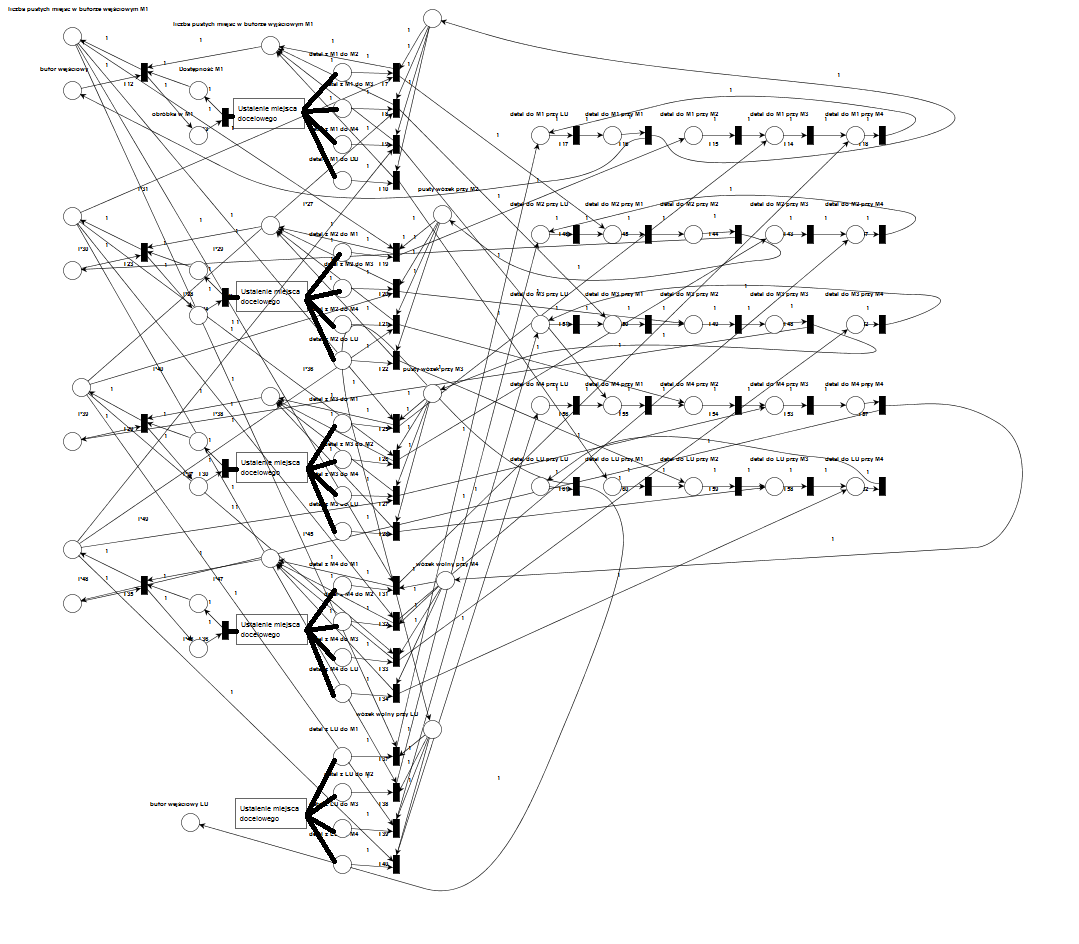
\includegraphics[width=1\textwidth]{./obrazki/Petri.png}
    \caption{Sieć Petriego}
    \label{fig:petri}
  \end{center}
 \end{figure}
Wykorzystaliśmy standardowe oznaczenia miejsc i tranzycji w sieciach Petriego. Wyróżniliśmy operacje maszynowe oraz realizowane przez wózki AGV, które są obserwowalne przez sterownik główny, po zakończeniu danego zadania maszyna/wózek informuje o tym kontroler główny, który może zlecić nowe zadanie dla maszyny/wózka (zdarzenie kontrolowalne).

\section{Plan pracy i rozkład w czasie}
\label{sec:org}

Na rysunku~\ref{fig:gantt} znajdują się wyselekcjonowane zadania oraz czas ich trwania jak również zaznaczone zostały kamienie milowe. 
 \begin{figure}[H]
  \begin{center}
    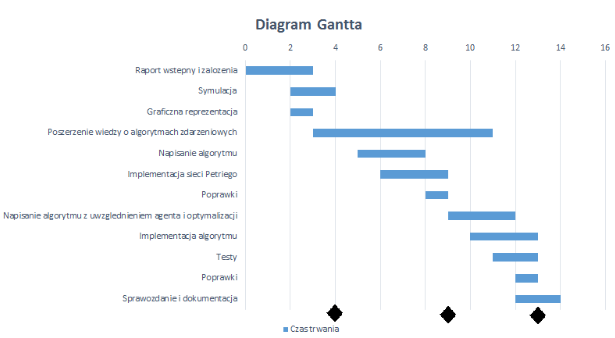
\includegraphics[width=1\textwidth]{./obrazki/gantt.png}
    \caption{Diagram Gantta}
    \label{fig:gantt}
  \end{center}
 \end{figure}

\section{Zarządzanie projektem}

Spotkania zespołu odbywać się będą w terminie zajęć oraz po wcześniejszym umówieniu się członków zespołu przy użyciu \textit{Skype’a} oraz grupy na portalu społecznościowym \textit{Facebook}. Oficjalnym liderem grupy jest Hanna Sienkiewicz. Jest to osoba, która jest odpowiedzialna za rozliczanie z zadań członków grupy przed upływem wyznaczonych terminów. Podział zadań w grupie następuje zgodnie z umiejętnościami i oczekiwaniami poszczególnych członków grupy. Nie przewidujemy problemów z tym związanych, członkowie grupy czują się zobligowani do pomocy przy większych i trudniejszych zadaniach. 

\section{Zespół}

W skład zespołu projektowego wchodzą
\begin{itemize}
\item Hanna Sienkiewicz, lider grupy, dane kontaktowe: 184184@student.pwr.edu.pl,
\item Marcin Ciopcia,
\item Daniel Gut,
\item Piotr Semberecki,
\item Mateusz Stachowski.
\end{itemize}

\section{Struktura systemu}

W systemie zdarzeniowym można wyróżnić
\begin{itemize}
\item sterownik główny,
\item sterowniki maszyn,
\item sieć Petriego,
\item symulator zdarzeń.
\end{itemize}

Symulator ma za zadanie zasymulować uruchomienie zadania na maszynie, ładowanie z bufora do maszyny oraz ładowania z maszyny na wózek.

Pierwszy model sterownika działa na zasadzie wykonywania zadań jako pierwszych, których suma czasów wykonywania poszczególnych etapów jest najmniejsza. Posiada on wiedzę o zadaniach, jakie mogą być wykonane w danym kroku czasowym oraz o maszynach, na których będą wykonywane poszczególne etapy zadania jaki o czasach wykonania poszczególnych etapów zadania.


%Sieć (P/T Sieć) formalnie można zapisać za pomocą piątki $N\ =\ (P,\ T,\ F,\ W,\ M_0)$, gdzie:
%\begin{itemize}
%\item $P$ jest skończonym zbiorem miejsc,
%\item $T$ jest skończonym zbiorem przejść (tranzycji),
%\item $P \cap T =\ \{\o \}$ - zbiory miejsc i przejść są rozłączne,
%\item $F \subseteq (P\times T)\cup (T\times P)$ jest relacją przepływu,
%\item $W:F\to (\mathcal{N}-\{0\})$ jest funkcją wagi łuków,
%\item $M_0:P  \to \mathcal{N}$ jest markowaniem początkowym.
%\end{itemize}
%\section{Sekwencyjny system alokacji zasobów}
%
%RAS definiuje się jako piątkę $\Phi \ =\ (\mathcal{R},\ C,\ \mathcal{P},\ \mathcal{D},\ \mathcal{T})$, gdzie:
%\begin{itemize}
%\item $\mathcal{R}$ jest zbiorem typów zasobów,
%\item $C$ jest funkcją pojemności zasobów,
%\item $\mathcal{P}$ - jest zbiorem typów procesów,
%\item $F \subseteq (P\times T)\cup (T\times P)$ jest relacją przepływu,
%\item $W:F\to (\mathcal{N}-\{0\})$ jest funkcją wagi łuków.
%\item $\mathcal{R}=\{M_i,\ B_{wy_i},\ B_{we_i},\ L/U,\ AGV_j,\ W_j\}$, $i=1,\dots 4,\ j=1,\dots, 4$, gdzie $M$ - zasób maszynowy, $B$ - zasób buforowy, $L/U$ - zasób stacji, $AGV$ - zasób wózków, $W$ - zasób wolnego miejsca między maszynami.
%\item $C(M_i)=1,\ C(B_{we_i})=x,\ C(B_{wy_i})=y,\ C(AGV_i)=z,\ C(L/U)=\infty,\ C(W_j)=w;\ x,\ y,\ z,\ w$ - parametry,
%\item $\mathcal{P}=\{\Pi_i\}$, $i=1,\dots, 6$, (6 procesów to 6 typów produktów),
%\item $\Pi_j=\big<\mathcal{S}_j,\mathcal{G}_j\big>$,
%\item $\mathcal{S}_j=\{Om_{j1},\dots ,Om_{jn(j)}, Ow_{j1},\dots ,Ow_{jm(j)} \}$ zbiór operacji procesu $\Pi_j$, $Om$ - operacje maszynowe, $Ow$ - operacje transportowe,
%\item $\mathcal{G}_j=\{O, t\}$ jest strukturą danych wyznaczającą logikę wykonywania operacji procesu $\Pi_j$; $O$ to zbiór operacji, $t$ czas operacji $O$
%\item $\mathcal{D}:$  jest funkcją wymagań zasobowych operacji, operacje transportu wymagają dostępności wózków oraz wolnej ścieżki między danymi maszynami, operację maszynowe wymagają miejsca w buforze wejściowym oraz wyjściowym jaki i dostępności maszyny; np. $D_{11}=\{B_we1,\ M_1,\ B_wy1\}$ - wymagania zasobowe operacji maszynowej $Om_{11}$.
%
%
%\end{itemize}
%SU-RAS, w którym funkcja wymagań zasobowych jest określona przez D. Każda operacja $O$ wymaga jednej jednostki jednego typu zasobu.
%
%Jeżeli detal musi zostać przewieziony z bufora wyjściowego maszyny X na bufor wejściowy maszyny Y to żąda on wolnego miejsca na trasie miedzy tymi maszynami i jednocześnie wózka, który go przewiezie, to oznacza, że jeżeli wózek i wolne miejsce na trasie to zasoby to operacja transportu wymaga dwóch jednostek zasobów różnych typów (każda operacja wymaga jednej jednostki jednego typu zasobu).

\section{Unikanie blokad}
W celu uniknięcia blokad stosujemy pojemność buforów wejściowych i wyjściowych maszyn większą niż 1. Zastosowaliśmy również w sterowniku głównym algorytm bankiera, który służy do sprawdzenia, czy dany stan jest bezpieczny, jeżeli tak to sterownik pozwala na realizację danego zadania, które doprowadza sieć do tego stanu bezpiecznego. Algorytm ten polega na skonstruowaniu ciągu bezpiecznego, tzn. takiego ciągu procesów $P(1),P(2),...,P(n)$, w którym proces $P(i)$ żąda zasobów wolnych w danym stanie lub zajętych przez procesy począwszy od $P(1)$ do $P(i-1)$. 



\section{Opis sterowania}
Rysunek nr~\ref{fig:alg} przedstawia działanie modelu zdarzeniowego.
 \begin{figure}[H]
  \begin{center}
    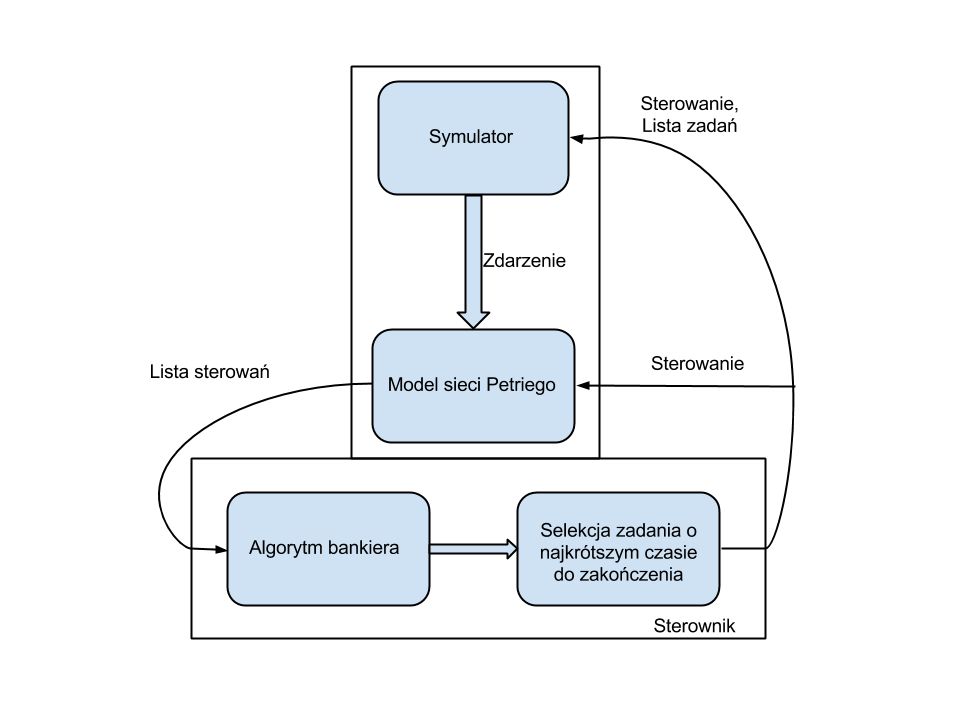
\includegraphics[width=1\textwidth]{./obrazki/alg.png}
    \caption{Architektura sterownika}
    \label{fig:alg}
  \end{center}
 \end{figure}
\subsection{Inicjalizacja zadań}
Zadanie to struktura wchodząca w skład listy zadań składająca się z
\begin{itemize}
\item  numerów maszyn, na których są wykonywane poszczególne etapy zadań\\
\textit{Lista\_zadan(i).maszyny = [$M_j$, $\dots$,  $M_n$]},
\item czasów obróbki jednego detalu na maszynie\\
\textit{Lista\_zadan(i).czasy = [$t_j$, $\dots$,  $t_n$]},
\item liczby detali oczekujących na obróbkę na maszynie\\
\textit{Lista\_zadan(i).ilosc   = [k, $\dots$, 0]}.
\label{lista_zad}
\end{itemize}
\subsection{Sterownik}
Sterownik na podstawie listy dostępnych sterowań wygenerowanych przez model sieci Petriego, listy zadań oraz wielkości buforów wyjściowych i wejściowych maszyn generuje \textbf{Sterowanie}. \textbf{Sterowanie} to struktura zawierająca w sobie
\begin{itemize}
\item typ zadania (typy zadań zostały opisane w sekcji~\ref{funkcje}),
\item numer maszyny - określa nr maszyny, przy której zdarzenie wystąpiło,
\item numer - to numer zadania z listy zadań,
\item etap - to numer etapu zadania.
\end{itemize}
Sterowanie generowane jest poprzez algorytm bankiera, następnie z pośród możliwych zadań wybierane jest to, które ma najkrótszy czas do zakończenia. Algorytm bankiera jest zaimplementowany dla maszyn z zadania.  Agent przyjmuje jako parametry
\begin{itemize}
\item listę dostępnych sterowań wygenerowaną przez model sieci Petriego, zawierającą możliwe \textbf{Sterowania},
\item listę zadań.
\end{itemize}
Do sterowania przejazdem wózków wydzielamy osobną warstwę w sterowniku - Sterownik transportu. Sterownik nadrzędny po wybraniu następnego zadania przekazuje je do warstwy sterowania transportem. Następnie sterownik od transportu bierze aktualny etap zadania (w celu ustalenia skąd ma wziąć detal) i następny etap zadania, aby ustalić dokąd ma trafić detal. Jeżeli detal znajduje się przy maszynie $1$-ej i chcemy żeby trafił do maszyny $4$-tej to począwszy od miejsca $1$-tego w przeciwnym kierunku niż ruch wózków Sterownik transportowy szuka pierwszego, wolnego wózka. Jeżeli okazało by się, że przy miejscu $4$-tym nie ma wolnych wózków to przesuwamy go o jeden do przodu (oczywiście przy większej liczbie powstanie rekurencja).
\subsection{Symulator}
W symulatorze można rozróżnić symulator maszyn i symulator wózków. Główne zadania symulatora to
\begin{itemize}
\item przeniesienie detalu z bufora wyjściowego maszyny na wózek i zasymulowanie ruchu tego wózka,
\item zatrzymanie wózka przy maszynie i przeniesienie detalu do bufora wejściowego maszyny,
\item przeniesienie detalu z bufora wyjściowego do gniazda obróbczego,
\item przeniesienie detalu z gniazda obróbczego do bufora wyjściowego,
\end{itemize}
Każde z tych zdarzeń trwa określoną jednostkę czasu.
\subsection{Model sieci Petriego - opis stanu sieci}
Stan sieci to macierz rozmiaru $13$x$ 5$. Stan początkowy wygląda następująco
\begin{equation}
\left[\begin{array}{ccccc}
0 & 0 & 0 & 0&0\\
0 &0 &0 &0&0\\
0 &0 &0 &0&0\\
0 &0 &0 &0&0\\
0 &0 &0 &0&0\\
0 &0 &0 &0 &1\\
0 &0 &0 &0&0\\
b_{we}&b_{we}&b_{we}&b_{we} & \infty\\
b_{wy}&b_{wy}&b_{wy}&b_{wy} & \infty\\
1&1&1&1 &1\\
0 &0 &0 &0 &0\\
0 &0 &0 &0 &0\\
0 &0 &0 &0 &0
\end{array}\right],
\end{equation}
gdzie $b_{we}$, $b_{wy}$ to odpowiednio rozmiar bufora wejściowego i wyjściowego, a
\begin{itemize}
\item 1. wiersz sieci to transport do maszyny 1,
\item 2. wiersz sieci to transport do maszyny 2,
\item 3. wiersz sieci to transport do maszyny 3,
\item 4. wiersz sieci to transport do maszyny 4,
\item 5. wiersz sieci to transport do LU,
\item 6. wiersz sieci to oznaczenie miejsca z pustym wózkiem (domyślnie jeden pusty wózek przy LU),
\item 7. wiersz sieci to ilość detali w buforach wejściowych (domyślnie zero dla każdej maszyny),
\item 8. wiersz sieci to liczba pustych miejsc w buforach wejściowych dla każdej z maszyn,
\item 9. wiersz sieci to liczba pustych miejsc w buforach wyjściowych dla każdej z maszyn,
\item 10. wiersz sieci to dostępność maszyn (domyślnie wszystkie maszyny są dostępne),
\item 11. wiersz sieci to obróbka na maszynie,
\item 12. wiersz sieci to wózek w ruchu miedzy M1 a M2, M2 a M3, M3 a M4, M4 a LU, LU a M1 (domyślnie żaden wózek nie jest w ruchu),
\item 13. wierz sieci to gotowy detal do odbioru znajdujący się w buforze wyjściowym maszyny (domyślnie nie ma gotowych detali).
\end{itemize}
Przykładowo transport do maszyny nr 4 z maszyny nr 3 to S[4][3]=1 oraz S[12][3]=1 (wózek w ruchu). Po wykonaniu tego transportu mamy S[4][3]=0, S[4][4]=1 oraz S[12][3]=0.
\subsubsection{Symulacja zdarzeń i sterowań w modelu sieci Petriego}
\label{funkcje}

Tutaj zostało opisane działanie sieci Petriego wraz z obrazującym to działanie przykładem.
\newline
Istnieją 4 typy zadań
\begin{itemize}

\item Typ 3 - Załaduj wózek,
Zgłaszamy, że detal nie jest już w gnieździe maszyny, maszyna ta staje się dostępna. Sprawdzamy czy mamy pusty wózek przy maszynie $i$ czy jest miejsce w buforze wejściowym maszyny docelowej. Jeśli tak to rezerwujemy wózek. Zmniejszamy liczbę dostępnych miejsc w buforze wejściowym maszyny docelowej o 1. Zwiększamy miejsce w buforze wejściowym dla maszyny, która opuszcza detal. W wierszu o numerze maszyny docelowej, zaznaczamy transport do niej począwszy od maszyny aktualnej. W takim stanie możliwy jest transport. Do \textbf{Listy dostępnych zadań} dodawane jest \textbf{Sterowanie} - transport.
\begin{equation*}
S_1=\left[\begin{array}{ccccc}
0 & 0 & 0 & 0&0\\
0 & 0 & 0 & 0 & 0\\
0 & 0 & 0 & 0& 0\\
0 & 0 & 0 & 0& 0\\
0 & 0 & 0 & 0& 0\\
1 & 0 & 0 & 0 & 0\\
0 & 0 & 0 & 0& 0\\
b_{we}& b_{we}& b_{we}& b_{we} & \infty\\
b_{wy}& b_{wy}& b_{wy}& b_{wy} & \infty\\
0& 1& 1& 1 & 1\\
1 & 0 & 0 & 0 & 0\\
0 & 0 & 0 & 0 & 0\\
0 & 0 & 0 & 0 & 0
\end{array}\right],
\end{equation*}
$S_1[6][1]=1$ jest pusty wózek przy maszynie nr 1. Żaden wózek nie jest w ruchu. $S_1[10][1]=0$ maszyna M1 nie jest dostępna, ponieważ $S_1[11][1]=1$ obróbka detalu trwa. $S_1[8][3]>0$ bufor wejściowy maszyny docelowej M3 nie jest pełny. Symulator po czasie trwania obróbki detalu na maszynie M1 zgłasza \textbf{Zdarzenie} do sieci o przeniesienie tego detalu do bufora wyjściowego tej maszyny.
\begin{equation*}
S_2=\left[\begin{array}{ccccc}
0 & 0 & 0 & 0&0\\
0 & 0 & 0 & 0 & 0\\
0 & 0 & 0 & 0& 0\\
0 & 0 & 0 & 0& 0\\
0 & 0 & 0 & 0& 0\\
1 & 0 & 0 & 0 & 0\\
0 & 0 & 0 & 0& 0\\
b_{we}& b_{we}& b_{we}& b_{we} & \infty\\
b_{wy}& b_{wy}& b_{wy}& b_{wy} & \infty\\
1& 1& 1& 1 & 1\\
0 & 0 & 0 & 0 & 0\\
0 & 0 & 0 & 0 & 0\\
1 & 0 & 0 & 0 & 0
\end{array}\right],
\end{equation*}
$S_2[13][1]$=1 - gotowy detal do odbioru w buforze wyjściowym maszyny M1. $S_2[11][1]=0$ obróbka zakończona, $S_2[10][1]=1$ - maszyna M1 znów dostępna. Po zgłoszeniu \textbf{Zdarzenia}- Załaduj wózek mamy
\begin{equation*}
S_3=\left[\begin{array}{ccccc}
0 & 0 & 0 & 0&0\\
0 & 0 & 0 & 0 & 0\\
1 & 0 & 0 & 0& 0\\
0 & 0 & 0 & 0& 0\\
0 & 0 & 0 & 0& 0\\
0 & 0 & 0 & 0 & 0\\
0 & 0 & 0 & 0& 0\\
b_{we}& b_{we}& b_{we}-1& b_{we} & \infty\\
b_{wy}+1& b_{wy}& b_{wy}& b_{wy} & \infty\\
1& 1& 1& 1 & 1\\
0 & 0 & 0 & 0 & 0\\
0 & 0 & 0 & 0 & 0\\
0 & 0 & 0 & 0 & 0
\end{array}\right],
\end{equation*}
$S_3[13][1]$=0 - detal został zabrany z bufora wyjściowego. $S_3[6][1]=0$ rezerwujemy wózek. $S_3[3][1]=1$ zaznaczamy transport z maszyny nr 1 na maszynę docelową (nr 3). $S_3[8][3]=b_{we}-1$ zmniejszamy liczbę dostępnych miejsc w buforze wejściowym maszyny docelowej. $S_3[9][1]=b_{wy}+1$ zwiększamy liczbę dostępnych miejsc w buforze wyjściowym maszyny nr 1. Możliwe jest \textbf{Sterowanie} - transport (dodawane do \textbf{Listy dostępnych zadań}).
\item Typ 2 - Wykonaj transport
\begin{equation*}
S_4=\left[\begin{array}{ccccc}
0 & 0 & 0 & 0& 0\\
0 & 0 & 0 & 0 & 0\\
1 & 0 & 0 & 0& 0\\
0 & 0 & 0 & 0& 0\\
0 & 0 & 0 & 0& 0\\
0 & 0 & 0 & 0 & 0\\
0 & 0 & 0 & 0& 0\\
b_{we}& b_{we}& b_{we}& b_{we} & \infty\\
b_{wy}& b_{wy}& b_{wy}& b_{wy} & \infty\\
1& 1& 1& 1 & 1\\
0 & 0 & 0 & 0 & 0\\
1 & 0 & 0 & 0 & 0\\
0 & 0 & 0 & 0 & 0
\end{array}\right],
\end{equation*}
Symulator wystawia zdarzenie ruchu wózka $S_4[12][1]$ - wózek w ruchu między M1 a M2.
\begin{equation*}
S_5=\left[\begin{array}{ccccc}
0 & 0 & 0 & 0& 0\\
0 & 0 & 0 & 0 & 0\\
0 & 1 & 0 & 0& 0\\
0 & 0 & 0 & 0& 0\\
0 & 0 & 0 & 0& 0\\
0 & 0 & 0 & 0 & 0\\
0 & 0 & 0 & 0& 0\\
b_{we}& b_{we}& b_{we}& b_{we} & \infty\\
b_{wy}& b_{wy}& b_{wy}& b_{wy} & \infty\\
1& 1& 1& 1 & 1\\
0 & 0 & 0 & 0 & 0\\
0 & 0 & 0 & 0 & 0\\
0 & 0 & 0 & 0 & 0
\end{array}\right],
\end{equation*}
$S_5[12][1]$=0 - koniec ruchu miedzy M1 a M2. Symulator wystawia \textbf{Zdarzenie} - $S_5[3][1]=0$ został wykonany transport z maszyny nr 1 na maszynę nr 2, dalej wykonujemy \textbf{Zdarzenie} - transport z maszyny nr 2 na maszynę nr 3, $S_5[3][2]=1$.
\begin{equation*}
S_6=\left[\begin{array}{ccccc}
0 & 0 & 0 & 0&0\\
0 & 0 & 0 & 0 & 0\\
0 & 1 & 0 & 0& 0\\
0 & 0 & 0 & 0& 0\\
0 & 0 & 0 & 0& 0\\
0 & 0 & 0 & 0 & 0\\
0 & 0 & 0 & 0& 0\\
b_{we}& b_{we}& b_{we}& b_{we} & \infty\\
b_{wy}& b_{wy}& b_{wy}& b_{wy} & \infty\\
1& 1& 1& 1 & 1\\
0 & 0 & 0 & 0 & 0\\
0 & 1 & 0 & 0 & 0\\
0 & 0 & 0 & 0 & 0
\end{array}\right],
\end{equation*}
Symulator wystawia \textbf{Zdarzenie} - ruch wózka między M2 a M3 -$S_6[12][2]=1$.
\begin{equation*}
S_7=\left[\begin{array}{ccccc}
0 & 0 & 0 & 0&0\\
0 & 0 & 0 & 0 & 0\\
0 & 0 & 1 & 0& 0\\
0 & 0 & 0 & 0& 0\\
0 & 0 & 0 & 0& 0\\
0 & 0 & 0 & 0 & 0\\
0 & 0 & 0 & 0& 0\\
b_{we}& b_{we}& b_{we}& b_{we} & \infty\\
b_{wy}& b_{wy}& b_{wy}& b_{wy} & \infty\\
1& 1& 1& 1 & 1\\
0 & 0 & 0 & 0 & 0\\
0 & 0 & 0 & 0 & 0\\
0 & 0 & 0 & 0 & 0
\end{array}\right],
\end{equation*}
Po czasie jazdy wózka symulator informuje sieć o \textbf{Zdarzeniu} - koniec ruchu wózka $S_7[12][2]=0$, $S_7[3][2]=0$ - został wykonany transport z maszyny nr 2 na maszynę nr 3. Następnie sieć wykonuje \textbf{Zdarzenie} - załadunek do bufora wejściowego maszyny nr 3 - $S_7[3][3]=1$.
\begin{equation*}
S_8=\left[\begin{array}{ccccc}
0 & 0 & 0 & 0& 0\\
0 & 0 & 0 & 0 & 0\\
0 & 0 & 0 & 0& 0\\
0 & 0 & 0 & 0& 0\\
0 & 0 & 0 & 0& 0\\
0 & 0 & 1 & 0 & 0\\
0 & 0 & 1 & 0& 0\\
b_{we}& b_{we}& b_{we}& b_{we} & \infty\\
b_{wy}& b_{wy}& b_{wy}& b_{wy} & \infty\\
1& 1& 1& 1 & 1\\
0 & 0 & 0 & 0 & 0\\
0 & 0 & 0 & 0 & 0\\
0 & 0 & 0 & 0 & 0
\end{array}\right],
\end{equation*}
$S_8[3][3]=0$, $S_8[6][3]=1$ mamy pusty wózek przy maszynie nr 3, $S_8[7][3]=1$ mamy detal w buforze wejściowym maszyny nr 3. Zgłaszamy możliwość \textbf{Sterowania} - załadunek detalu na maszynę.

\item Typ 1 - Załaduj detal na maszynę. Jeśli jest to ostatni etap zadania i maszyna docelowa to LU, to zadanie zostaje zakończone. Zgłaszamy pusty wózek. Zwiększamy liczbę miejsc w buforze wejściowym maszyny o 1. Zgłaszamy \textbf{Sterowanie} - możliwość obróbki (do \textbf{Listy dostępnych zadań}).
\begin{equation*}
S_9=\left[\begin{array}{ccccc}
0 & 0 & 0 & 0&0\\
0 & 0 & 0 & 0 & 0\\
0 & 0 & 0 & 0& 0\\
0 & 0 & 0 & 0& 0\\
0 & 0 & 0 & 0& 0\\
0 & 0 & 1 & 0 & 0\\
0 & 0 & 0 & 0& 0\\
b_{we}& b_{we}& b_{we}+1& b_{we} & \infty\\
b_{wy}& b_{wy}& b_{wy}& b_{wy} & \infty\\
1& 1& 1& 1 & 1\\
0 & 0 & 0 & 0 & 0\\
0 & 0 & 0 & 0 & 0\\
0 & 0 & 0 & 0 & 0
\end{array}\right],
\end{equation*}
$S_9[8][3]=b_{we}+1$ zwiększamy liczbę miejsc w buforze wejściowym maszyny o 1. $S_9[7][3]=0$ - jest to \textbf{Zdarzenie} przeniesienie z bufora wejściowego maszyny nr 3 do jej gniazda obróbczego.


\item Typ 4 - Wykonaj obróbkę.
Do odpowiedniej kolumny wiersza 11 jest wpisywana jedynka.
\begin{equation*}
S_{10}=\left[\begin{array}{ccccc}
0 & 0 & 0 & 0&0\\
0 & 0 & 0 & 0 & 0\\
0 & 0 & 0 & 0& 0\\
0 & 0 & 0 & 0& 0\\
0 & 0 & 0 & 0& 0\\
0 & 0 & 1 & 0 & 0\\
0 & 0 & 0 & 0& 0\\
b_{we}& b_{we}& b_{we}& b_{we} & \infty\\
b_{wy}& b_{wy}& b_{wy}& b_{wy} & \infty\\
0 & 1& 1& 1 & 1\\
1 & 0 & 0 & 0 & 0\\
0 & 0 & 0 & 0 & 0\\
0 & 0 & 0 & 0 & 0
\end{array}\right],
\end{equation*}
\textbf{Zdarzenie} - $S_{10}[11][3]=1$ trwa obróbka na maszynie nr 3. $S_{10}[10][3]=0$ maszyna nr 3 nie jest wolna. 
\begin{equation*}
S_{11}=\left[\begin{array}{ccccc}
0 & 0 & 0 & 0&0\\
0 & 0 & 0 & 0 & 0\\
0 & 0 & 0 & 0& 0\\
0 & 0 & 0 & 0& 0\\
0 & 0 & 0 & 0& 0\\
0 & 0 & 1 & 0 & 0\\
0 & 0 & 0 & 0& 0\\
b_{we}& b_{we}& b_{we}& b_{we} & \infty\\
b_{wy}& b_{wy}& b_{wy}& b_{wy} & \infty\\
1 & 1& 1& 1 & 1\\
0 & 0 & 0 & 0 & 0\\
0 & 0 & 0 & 0 & 0\\
0 & 0 & 1 & 0 & 0
\end{array}\right],
\end{equation*}
Po upłynięciu czasu obróbki, symulator wystawia \textbf{Zdarzenie} - przeniesienie detalu z gniazda obróbczego do bufora wyjściowego maszyny. $S_{11}[13][3]=1$ - gotowy detal w buforze wyjściowym maszyny M3. $S_{11}[11][3]=0$ - koniec obróbki na maszynie M3, $S_{11}[10][3]=1$ - maszyny M3 jest wolna. Zgłaszamy możliwość \textbf{Sterowania} - załadunek wózka (do \textbf{Listy dostępnych zadań}), po wykonanej obróbce.
\end{itemize}
\section{Struktura programu}
\begin{itemize}
\item AlgBankiera.m funkcja zawierająca algorytm bankiera,
\item IleZadanNaLiscie.m funkcja liczy ile zadań pozostało do realizacji na danej $Liście\ Zadań$,
\item PetriNet.m klasa implementująca sieć Petriego,
\item Sterowanie.m klasa implementuje pojedyncze zdarzenie sterowania,
\item Zadanie.m klasa implementuje zadanie do zrealizowania przez system zdarzeniowy,
\item agent.m funkcja implementuje agenta decyzyjnego sterownika zdarzeniowego,
\item agvInit.m funkcja implementuje wózek AGV jak strukturę,
\item loadOnInputBuf.m 	funkcja implementuje wrzucenie detalu na bufor wejściowy maszyny,
\item loadOnMachineSocket.m funkcja implementuje wrzucenie detalu na gniazdo obróbcze maszyny,
\item loadOnOutputBuf.m funkcja implementuje wrzucenie detalu na bufor wyjściowy maszyny,
\item machineInit.m funkcja inicjuje maszyny jako struktury danych,
\item main.m program emuluje działanie robotycznego systemu obróbczego w orientacji kołowej oraz implementuje sterownik zdarzeniowy zarządzający siecią,
\item simInit.m inicjalizacja symulatora.
\end{itemize}
\subsection{Główna pętla programu}
Przykładowa inicjalizacja zadań jest następująca
\begin{lstlisting}[language=Matlab, frame=single,tabsize=1, caption={Inicjalizacja zadań w pliku main.m}]
Lista_zadan(1).maszyny = [ 1, 2, 3];
Lista_zadan(1).czasy = [ 20, 8, 35];
Lista_zadan(1).ilosc = [ 5, 0, 0];
Lista_zadan(2).maszyny = [ 2, 1, 2, 3];
Lista_zadan(2).czasy = [ 7, 14, 5, 40];
Lista_zadan(2).ilosc = [ 5, 0, 0, 0];
IleZadanNaStart = IleZadanNaLiscie(Lista_zadan);
IleZadanW_U = 0;
\end{lstlisting}
Główna pętla programu z wyszczególnionymi symulatorem siecią Petriego oraz sterownikiem.
\begin{lstlisting}[language=Matlab, frame=single,tabsize=1, caption={Część pliku main.m}]
while(IleZadanW_U < IleZadanNaStart)
% iteruj symulator
Zdarzenie = AktualizujSymulator( Sterowanie, Lista_zadan );
% jesli Sterowanie = [] to iteruj do nastepnego zdarzenia
% iteruj siec petriego
Lista_sterowan = PetriNet.AktulaizujOZdarzenie( Zdarzenie);
% selekcja zadan
Sterowanie = agent(Petri.listaDostepnychSterowan(),
/Lista_zadan,Wielkosc_buforow);
% aktualizowanie sieci w oparciu o Sterowanie
Petri.wykonajSterowanie(Sterowanie);
end
\end{lstlisting}
\begin{thebibliography}{9}
\bibitem{scr}
  S. Samolej, B. Trybus,
  \emph{Zastosowanie kolorowanych sieci Petriego w projektowaniu systemów czasu rzeczywistego}.
  Pomiary, Automatyka, Kontrola,
  2005,
  tom R. 51, nr 1,
  11-13.
\bibitem{sl}  
  I. Grobelna, M. Grobelny,
  \emph{Projektowanie sterowników logicznych z wykorzystaniem łuków zezwalających i zakazujących sieci Petriego}.	
  Pomiary, Automatyka, Kontrola,
  2012,
  tom R. 58, nr 7,
  605-607.
  
 \bibitem{mucha} 
  G. Bocewicz, W. Muszyński, Z. Banaszak,
  \emph{Modele multimodalnych sieci i procesów transportowych}.
  Postępy robotyki pod redakcją K. Tchonia i C. Zielińskiego,
  Oficyna wydawnicza Politechniki Warszawskiej,
   Warszawa 2014,
   tom 2, s. 543-552.

\end{thebibliography}

\end{document}


 
